% !TeX root = ../main.tex
% Add the above to each chapter to make compiling the PDF easier in some editors.

\chapter{Creation of new models}\label{chapter:Models}
To improve the simulation and control of tendon-driven robots, new robot models were created and processed, such that the MyoMuscle plug-in can be added to them. These new robot models can be used to advance the simulation, such that it can be used for studying the human brain or body in the future. The following chapter presents how new robot models are created for the simulation by using tools provided by the NRP.

\section{Creation and Export of 3D Models}
New 3D models for the Roboy project are created in Autodesk Fusion 360. To use them in Gazebo, the models have to be converted to SDFormat files. As Autodesk Fusion 360 does not export to SDFusion files\footnote{\url{https://knowledge.autodesk.com/support/fusion-360/learn-explore/caas/sfdcarticles/sfdcarticles/How-to-export-a-design-in-Fusion-360.html}}, the SDFusion add-in is provided by the Roboy project and NRP. The latest version can be forwarded by a member of the Roboy simulation or the NRP team. To install the add-in, the SDFusion folder has to be added to the directory\footnote{\url{https://knowledge.autodesk.com/support/fusion-360/troubleshooting/caas/sfdcarticles/sfdcarticles/How-to-install-an-ADD-IN-and-Script-in-Fusion-360.html}}: \codew{\%appdata\%\textbackslash Autodesk\textbackslash Autodesk Fusion 360\textbackslash API\textbackslash AddIns}.%\footnote{\url{https://knowledge.autodesk.com/support/fusion-360/troubleshooting/caas/sfdcarticles/sfdcarticles/How-to-install-an-ADD-IN-and-Script-in-Fusion-360.html}}. 

First, already created 3D models were exported to the SDFormat using SDFusion, so that these models can be used to develop the simulation in the future. Furthermore, occurring problems were solved. Changes to the code can be found in appendix \ref{sec:code}. The following describes how to work with the SDFusion add-in.

Already existing and finished 3D models can be found in the Roboy Autodesk folder. To gain access to it, a member of the Roboy project should be contacted. Before working with the models, they have to be copied to the export\_model folder to keep the original models untouched.

%\begin{figure}[h]
%\centering
%   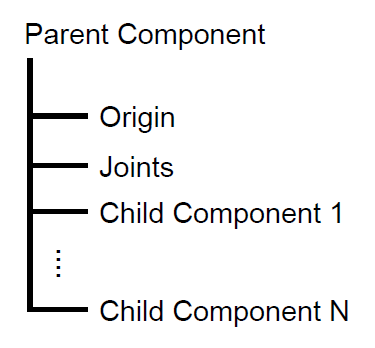
\includegraphics[width=0.33\textwidth] {figures/ADF.png}
%\label{fig:Autodesk}
%  \caption{Component structure in Autodesk Fusion 360}
%\end{figure}

Each Autodesk Fusion 360 3D model is an assembly of different components\footnote{\url{http://help.autodesk.com/view/fusion360/ENU/?learn=assemble}}. A component consists of an origin, child nodes and joints between child components. A child node can be a child component, but also a body or a spline. Each link has to be defined as a rigid group in Autodesk Fusion 360 and can be found in `Joints'.

The add-in can be found in the `add-in and scripts' window in the ‘model’ panel.  The edit option for SDFusion in the `Add-Ins' tab opens the code in a Spyder 2 environment, where it can be edited and run. Once the add-in is run, the save directory and root link are selected. The add-in first exports the root link and then recursively exports new links that are connected to already exported links by joints. Ideally, the root link should be a central link, e.g.\ the hip of the robot instead of a foot. For each link, every body belonging to it is copied and translated to the origin based on the joint it is connected to. Afterwards the duplicated, translated link is exported to a stl file and deleted. Then, nodes for the link and joint are written to the SDFormat file. For a large number of bodies, this requires a high computational cost.
 
As each link consists of several bodies, it is natural to merge all bodies belonging to the same link to reduce the computational cost for the export. The following provides a guide on how to merge bodies, problems that occurred and how to solve them as well as tips to simplify and accelerate the process.

To merge bodies of the same link, it is recommendable to first hide bodies belonging to other links. This ensures that unwanted bodies are not merged. A rigid group of the model can be checked in the ‘Browser’ window to determine the bodies belonging to it. `Selection by body priority' should be set, as it speeds up the selection process and selecting non-bodies, e.g.\ joints or splines, prevents joining. The ‘combine’ window can be opened by choosing `combine' under the ‘modify’ option of the ‘model’ panel. Running the command merges selected bodies. First, a target body has to be chosen. Every other selected body, the tool bodies, are merged to the target body. When merging bodies, they have to be connected, i.e.\ there has to be an intersection. The combine options ‘keep tools’ and ‘new component’ should normally be unchecked.

To merge bodies, it is possible to either preselect the bodies to merge and run the combine command afterwards or the other way around. Using the former method selects a target body arbitrary. Bodies can be selected by either selecting them individually or by creating a selection window around the desired bodies. Once the combine window is opened, selecting already selected bodies reverts the selection. As some bodies are inside others, they are not initially selectable. To solve this, all connected, selectable bodies should be merged first. For the next step, this merged body can be set as the target body and hid to select the bodies within. Thus, bodies sometimes have to be merged in several steps. This is desirable as Autodesk Fusion 360 might start to lag with large models if a large number of tool bodies are selected.

When merging bodies, it is possible that bodies duplicate and appear at a different position. A workaround is to select the central body if the link is symmetrical. Otherwise, a solution is to check ‘new component’ in the combine window. This saves the merged body to a new component, that then has to be moved to the right parent component. The ‘new component’ option should be unchecked for the next merge.

Another possible occurring problem is, that, when selecting a target body, some copies of that body cannot be selected as a tool body. This can be avoided by merging these bodies in a second step or, if this doesn’t work, by either keeping these as a single body or by merging the bodies in a new component. Similarly, if you select a body as a tool body, some copies of that body can become invisible but still selectable. Therefore, it is advisable to always merge these bodies in the same step.

Furthermore, bodies connected to a joint should not be merged, as the position of the joint cannot be determined by the SDFusion add-in in this case. If already merged, the respective combine entry in the time line should be deleted. Then all the bodies except the ones connected to a joint can be merged again.

Note, that depending on the PC that is used, merging bodies and running the add-in can be very time-consuming or even cause Autodesk Fusion 360  or the PC to crash. Smaller models can be exported within a few minutes while bigger ones need up to several hours. If the PC cannot handle the task, another one should be used.
%
%Once bodies are merged, empty components should be deleted, as the add-in goes through all components. However, if a warning appears that the to be deleted component is referenced in the time line, the component must not be deleted, as it leads to bodies being deleted.

Once all the bodies are merged, the add-in can be run. During the process, several problems occurred, of which some were solved. Changes to the code and problems that were solved can be found in appendix \ref{sec:code}. The following describes the problems that have yet to be solved.

First of all, the joint types that are supported by Autodesk Fusion 360\footnote{\url{http://help.autodesk.com/view/fusion360/ENU/?guid=GUID-8818AE31-958A-4A59-989B-9875A174C67A}} and those supported by the SDFormat\footnote{\url{http://sdformat.org/spec?elem=joint&ver=1.5}} are not equivalent. Some joint types in Autodesk Fusion 360 cannot be directly converted to the SDFormat. The joint types so far supported are revolute, ball, fixed and slider. The joint types cylindrical, pin-slot and planar are not yet supported. Therefore, when building new models in Autodesk Fusion 360, these joint types should be avoided, as changing an already defined joint to another type can cause the model to disarrange.

Another error that sometimes occurred was the root link not being recognized as a rigid group, even though it is recognized as one during the recursion when using a different root link. A workaround is to choose other links as the root link. If this doesn’t work, deleting and redefining the rigid group differently, e.g.\ using the child components rather than the parent component, can solve this problem. However, this is not guaranteed to work and therefore, the cause of this problem has yet to be found and fixed.

Furthermore, models with closed geometries, e.g.\ two links connected by at least two joints, are exported with duplicated links. A method to detect closed geometries to avoid this has to be developed.

In addition, all bodies should be part of a rigid group, especially those connected to a joint. Otherwise, the model cannot be exported completely.

Once the models are exported to SDFormat files, they can be reviewed in Gazebo. A guide on how to add the exported models to Gazebo can be found in appendix \ref{sec:Gaz}. Some models could not be exported correctly. All models are rotated and some links are translated wrongly in Gazebo. An overview can be found in table \ref{tab:model}.


\section{Add tendons to Models}
The models created by Autodesk Fusion 360 do not have tendons yet. To add them, the Blender plug-in BlenderRobotDesigner is required. It can be downloaded \footnote{\url{https://github.com/HBPNeurorobotics/BlenderRobotDesigner}} and installed by following the instructions in the README.rst file. If pip cannot be found, the following commands should be executed in the command line before trying again:
\code{sudo apt-get install python python-pip subversion\\
pip install --upgrade pip}

This plug-in uses Blender as a GUI. It is able to import the model from a SDFormat file, e.g.\ one created by the SDFusion add-in, and some other file formats, and export to a SDFormat file, a ROS package and some other file formats. Furthermore, tendons or muscles can be added with this plug-in. The HB tab that should appear once the blender plug-in is installed provides all tools of the plug-in.% If the tab cannot be found, go to File>User preferences>add-ons and check Editor:NRP Robot Designer.Once Blender is restarted, the HB tab should appear above the ‘Tool’ tab.

The ‘Import SDF – plain’ option of Files in the HB tab imports a SDFormat file of a model. The desired SDFormat file can be chosen and the model can be placed. 

As the models can be quite large, it can be desired to reduce the number polygons first. This command can be found under ‘Geometries’ in ‘Polygon Reduction’. A mesh, i.e.\ a link, and the desired ratio of triangles to reduce to can be set. The option ‘Apply to all meshes’ applies the reduction to all meshes of the robot model.

Once the model is of desired size, muscles can be added. New muscles, i.e.\ tendons, can be created and named in ‘Edit Muscles’ under ‘Muscles’. Then, path points can be defined. Path points are points, where the tendon comes upon the robot and interacts with it\cite{BA}. To add a path point, the cursor has to be placed at the desired location and ‘Add new pathpoint’ has to be chosen. This creates a numbered path point that can later be adapted in ‘Edit Muscles’. Each path point has to be attached to a link. The link has to be selected in ‘Attach pathpoints to segments’ and then the respective path point number has to be chosen. Finally, in ‘Muscle Characteristics’, several properties such as muscle type, muscle length and muscle dimension can be set.

Once all muscles are defined, the finished model can be exported to a ROS package with the ‘Export SDF – Ros package’ option of ‘Files’ . The model can be saved in a blend file so that it can be edited later if necessary. The export creates a folder with a muscles.osim file. The definition of the muscles can be found under the `objects' tag, see figure \ref{fig:osim}. This definition then has to be copied to the original SDFormat file created by SDFusion under the `plugin' tag for the MyoMuscle plug-in. Finally, the name of the muscle, e.g.\ Thelen2003Muscle, has to be changed to myoMuscle, see figure \ref{fig:sdf}. By following these steps, a tendon-driven robot model, that possesses the MyoMuscle plug-in, is created. This model can then be controlled as described in chapter \ref{chapter:Roboy}.

%Depending on your PC, there is a possibility of Blender lagging or models not being able to load due to overheating. I recommend loading all models and saving them to blend files each. That way, you can open any desired models in Blender by opening the respective blend file. 

Due to a lack of time and several problems occurring, tendons were not added to robot models during the work. One problem is models being loaded differently in Blender compared to Gazebo. This indicates, that some models are not imported correctly by the BlenderRobotDesigner plug-in. Due to wrongly imported models, it is not possible to add tendons to some models. Furthermore, models with closed geometries cannot be imported due to a recursion error.

In order to add tendons to the models created in Autodesk Fusion 360, these problems have to be solved first. Afterwards, the MyoMuscle plug-in can be added to these models as described above. These models can the be used to improve the simulation and control of tendon-driven robots and subsequently aid the research of the human body or brain.